\chapter{Results \& Evaluation} % Main chapter title

\label{chap:results} % Change X to a consecutive number; for referencing this chapter elsewhere, use \ref{ChapterX}

%\Large WRITE A LITTLE BIT ABOUT WHICH EXAMPLES ARE SHOWN. 
%\normalsize

In this section I will discuss a number of cases and snippets to showcase the results and behaviour of the implemented algorithm. This includes trade-offs, design choices and flaws. In this section the different reasons that cause problems in the final highlighters will become apparent as well as which parts are very useful for the process.

\section{Embedding scope information}
The system of embedding highlighting information established in \ref{sec:Pipeline} is quite literally used in the Rascal grammars. An example of this is included here as well as in the appendix (\ref{app:advancedGrammar:contexts}). A number of things become clear about this way of embedding information:
\begin{itemize}
\item[]\emph{Pros:}
\subitem 1. Assigning scopes in this manner is easy and intuitive. 
\item[]\emph{Cons:}
\subitem 1. Having to write the entire scope for every rule quickly becomes tedious. 
\subsubitem Especially for simple cases (E.G. \gram{MyKeywords}). 
\subitem 2. Unable to assign scopes to nested symbols that rascal views as one. 
\subsubitem For example: \gram{"+" and "-"} inside the last priority group of \gram{Expression} 
\subitem 3. Knowledge of what Rascal sees as one symbol and what not is required.
\subsubitem \gram{Identifier} has only 1 symbol on its right-hand side.
\end{itemize}
\pagebreak
\lstinputlisting[language=RascalGrammar, caption={The advanced example grammar with scope information}]{Code/grammars/RascalExp/RascalEx_withContexts.grammar} 
To make the process of scope assigning less tedious, one could add scopes on Symbol level as well as production level. In this way \gram{MyKeywords} could get one scope assigned instead of four times the same one. To circumvent the second issue, one has to rewrite parts of the grammar that are in specific need of colouring. This is not the end of the world, but not preferable. A better possible approach would be to allow the assigning of scopes to labels. Since labels can be found and assigned inside the nested symbols of a production. The third issue is not as much an issue in the sense that it obstructs the usefulness of the algorithm, however it represents the fact that the implementation is not very user-friendly towards beginners of Rascal.

\section{Simplifying the grammar}
Inside the project there is a module called \emph{ToPlainGrammar}. This module does the rewriting of a standard Rascal grammar to the plain form. Results of this can be viewed below. This is done in smaller snippets from larger grammars. 2 snippets are shown here, the Expression non-terminal of the grammar in the previous section. The second snippet shows a formulation for a list of declarations.\\
For a complete look at the pipeline one can look at appendix \ref{app:advancedGrammar} through \ref{app:pico}. There are two forms of the \textit{toPlainGrammar}-function, one that preserves the priority and one that does not. The first can be viewed in the appendices, the second is used here.

\pagebreak
\lstinputlisting[language=RascalGrammar, caption={Snippets showcasing the behaviour of \textit{ToPlainGrammar}}]{Code/grammars/results_simple.grammar}
As seen above the removal of unwanted features functions as it should. It properly rewrites regular structures into a set of non-terminals, terminals and productions. It also properly removes parse-tree altering structures on the rules as well as labels and some of the tags (last of these are removed in the \textit{ToStronglyRegular}-section). The original version did not account for \gram{layout}-symbols nor for parameterized tokens. These are all taken care of in this new implementation as well.

\subsection{Scope information}
The scope-information that is present in the grammar is saved in a proper manner. The contexts are saved as tags which are of type \data{Attr}. These end up being in the \data{\\prod(_,_,set[Attr] attributes)}. Therefore rewriting the rules to \data{\\prod(_,_,_) or \\choice(_,_)} does not cause any loss of information. The symbol rewriting does not cause loss of information, because everything that is seen by the parser as one token is rewritten to still be one token (E.G. \gram{syntax A = A (B C) \{D ","\}+ ;} has only 3 tokens). These are kept during this transformation and will be extracted from the "plain grammar" once requested by the algorithm.

\section{ToStronglyRegularGrammar}

\subsection{Grammar2Graph}
The method present that converted a grammar into a graph did not perform well enough and has been rewritten to recurse (deeper) into tokens in order to find the deepest symbols present. The function visits all right-hand side elements once. Therefore this conversion runs in linear time with the size of the total amount of symbols of the grammar (nested included).

\subsection{Kosaraju}
Below the set of components of the advanced example grammar (Rascal expression) as well as the strongly regular version are shown. As can be observed, \gram{keyword MyKeywords} is nowhere to be found. This is due to the fact that keywords are always excluded since they only serve as disambiguation constructs and never as real non-terminals. They could never be rewritten to other non-terminals because of the implementation of the Rascal-language.
\begin{lstlisting}
//Original version
set[set[Symbol]]: {
  {sort("Expression")},
  {layouts("MyLayout")},
  {lex("Identifier")},
}
//Strongly regular version
set[set[Symbol]]: {
  {
    sort("Expression"),
    sort("Expression_end")
  },
  {layouts("MyLayout")},
  {lex("Identifier")}
}
\end{lstlisting}

\pagebreak
\subsection{Mohri and Nederhof's transformation}
In appendix \ref{app:MohriGrammar} the example from the original paper is included together with the output this module produces. It has some meaningless productions, this is part of the algorithm and the rules that it produces. Self-loops of the type $\prodgr{A}{A}$ could be removed.\\
Below the advanced example grammar is shown again, it shows how \data{Expression} is rewritten into two non-terminals being \data{Expression and Expression_end}.
\lstinputlisting[language=RascalGrammar, caption={The strongly regular approximation of the advanced expression grammar (\ref{app:advancedGrammar:stronglyregular})}]{Code/grammars/RascalExp/stronglyRegular.grammar}
The implementation of Mohri and Nederhof's algorithm works for all the cases that were tested and shown in this thesis, however there is an edge-case that is not covered in the implementation. This throws a warning, so once someone meets this edge-case it will be noticed. The case is matched when a mutually recursive set of non-terminals is completely left-linear, but not right-linear. If all rules are left-linear then this set of rules should not be rewritten. However on converting this set of rules to a NFA the algorithm crashes because it uses the simple NFA-construction algorithm from a right-linear grammar. In order to circumvent this one could rewrite the left-linear sets to right-linear ones with the standard rewriting-algorithm. 




\pagebreak
\section{The \emph{Strongly Regular Grammar} to StateMachines} \label{sec:results:strReg2machines}
In the appendix a number of NFAs as well as DFAs are included for other grammars and tokens. Here is a DFA and corresponding grammar that show the results of the algorithm and some of its flaws. 

\lstinputlisting[language=RascalGrammar, caption={A grammar showing nested comments}]{Code/grammars/comments/comments.grammar}
\begin{figure}[h!]
	\centering
	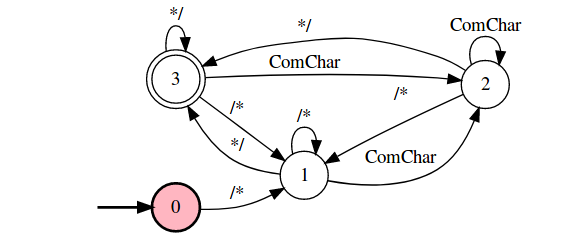
\includegraphics[width=\textwidth, keepaspectratio]{Figures/comment_dfa.png}
	\decoRule
 	\caption[DFA for Comment]{The DFA for Comment, produced from the strongly regular approximation}
\end{figure}
At first the machine seems proper, if one were to feed this a nested comment as input it is clear that it could consume this. This is good because it guarantees that there was no loss in information up till here. In terms of the algorithm and the final results however, this is a point which leads to problems in the final highlighter. When writing highlighters by hand, highlighting nested comments is easy because of the context-stack. The flow is simple: on opening comment push a comment context onto the stack, on closing comment pop a comment context off of the stack. The algorithm is designed in a different way, it creates a machine for each component and only pushes a machine if it finds a non-terminal on an arc such that when the pushed machine pops itself off, we end up in the next state. This ensures that within the machine above only the ComChar machine can be pushed, but never a nested comment machine. The choice made in \ref{sec:FinalStateCases} ensures that we remain in the same machine if we can in a non-sink state (state 3). Since a ComChar generally matches anything, so also code outside a comment, it chooses to remain in the machine forever. On top of that it is able to match as many opening and closing comments as it can without the need for balance. This means that the algorithm loses the possibility to properly highlight nested structures within the same component that require some sort of balancing (like bracket balancing and nested comments).

\section{The conflict resolution}
Implementing this part of the algorithm shows flaws in this step. It does however remove all conflicts in a machine except for the ones mentioned in \ref{sec:FinalStateCases}. These are similar to shift-reduce and reduce-reduce conflicts found in parsers.\\
The issues with this part of the algorithm are: 
\begin{enumerate}
\item This recursive process has a very bad time-complexity. It traverses all symbols in all components and all the transitions in the machines corresponding to these symbols. If a conflict is found, it runs the powerset-construction $NFA2DFA$-algorithm which has a bad time-complexity, and then reruns the search for conflicts.
\item Large grammars generate larger machines. Programming languages build on the recursive structure in a grammar and therefore a number of components tend to be large of size. This leads to enormous NFA's and DFA's. If conflicts arise, which happens at higher level tokens more often (like \gram{Statement} in C), the fixing of these conflicts cause large waiting times. This is due to the bad complexity (see the examples below).\\
Small example: x can be a variable or a function-call. Both have identifiers and are at the start of the statement, this will cause a conflict. 
\begin{lstlisting}[language=C]
void x() { printf("function x\n"); }
int main() {
	int x;
	x = 42;
	x(y);
}
\end{lstlisting}  
\item Another thing adding to the bad runtime of this algorithm is the fact that the machines of different symbols of the same component usually contain (many of) the same conflicts. These are all repetitively found and solved, including nested cases.
\end{enumerate}
\pagebreak
The reason the algorithm does not perform on large grammars is this part of the code. The amount of conflicts there are and that occur in a nested manner increase exponentially. Below is some output that was generated whilst working on the $C$ language in Rascal. It never finishes, but prints some statistics about where it is and what it is doing:

\begin{lstlisting}
	83/123: sort("Specifier__STARSEPS__TAIL_end")
sort("Specifier__STARSEPS__TAIL_end")
working on sort("Specifier__STARSEPS__TAIL_end"), currently with 314 conflicts
pre-nfa2dfa: current number of states: 1072
past nfa2dfa
past finding new conflicts
sort("Specifier__STARSEPS__TAIL_end")
working on sort("Specifier__STARSEPS__TAIL_end"), currently with 206 conflicts
pre-nfa2dfa: current number of states: 163
past nfa2dfa
past finding new conflicts
sort("Specifier__STARSEPS__TAIL_end")
working on sort("Specifier__STARSEPS__TAIL_end"), currently with 360 conflicts
pre-nfa2dfa: current number of states: 2038
past nfa2dfa
past finding new conflicts
\end{lstlisting}
This is the result of around 5 minutes of runtime on one of the tokens  it is handling. This was still a rather simple one because it resolved quickly, however there are 122 other tokens that also need conflict fixing which do not get solved this easily. This clearly shows just how unfeasible this approach is for large grammars. This is 1 machine out of 123 and it ends up with over 2000 states, meaning over 2000 contexts. A second example is a machine for the $Javascript$-grammar. It ran for 10 iterations like above and introduced more conflicts every step than there were resolved. At the 10th iteration it had 3544 conflicts and already 18688 states. After this I cancelled the operation as it took forever.



\section{ToContexts}
In this implementation, replacing an arc in a machine means that this non-terminal on this arc is gone afterwards. If a scope was assigned to this arc that information is lost from that point on, since it becomes part of this machine it will receive custom scopes in the next step of the algorithm. Therefore the highlighting might perform worse than expected. Implementation of this part proved harder since there was a lot of rewriting symbols into regular expressions involved. The information for this process was often not available at this point. Especially handling symbols that were of type \data{conditional(_,_)} proved difficult. There are no real intermediate results from this step as they tie together everything and produce the final highlighters to be discussed in the next section.

\pagebreak

\section{Resulting highlighters}
\subsection{Final results}
Together with an example performance the appendices now show the complete path that a grammar takes through the algorithm together with intermediate results. The results being: original grammar $\rightarrow$ plain grammar $\rightarrow$ strongly regular grammar $\rightarrow$ an example NFA constructed from this regular grammar $\rightarrow$ the corresponding DFA. Finally there is a small example program included in the form of a picture, showing the job the highlighter does. After this I have included the performance of a hand-written highlighter in a picture. The entire highlighters were not included for the very simple reason that they are all very long.\\

\noindent Rascal has a small DSL-like programming language called $Pico$. Pico is a 50 line grammar that generates 566 lines worth of highlighter. Besides the appendices the results of Pico are also included below. 
\begin{figure}[h!]
	\centering
	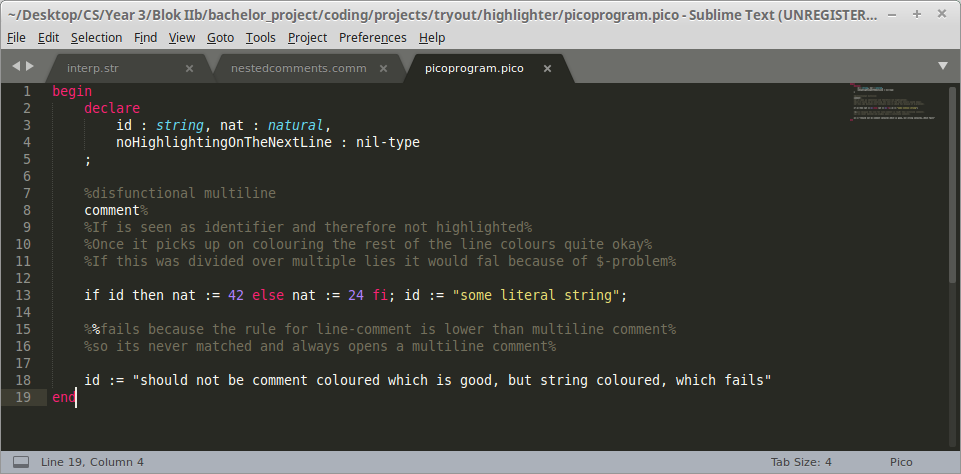
\includegraphics[width=\textwidth, keepaspectratio]{Figures/highlightShots/pico_generated.png}
	\decoRule
 	\caption[Generated highlighter results for Pico grammar]{Results of the highlighter generated for the pico grammar}
\end{figure}

\pagebreak
\begin{figure}[h!]
	\centering
	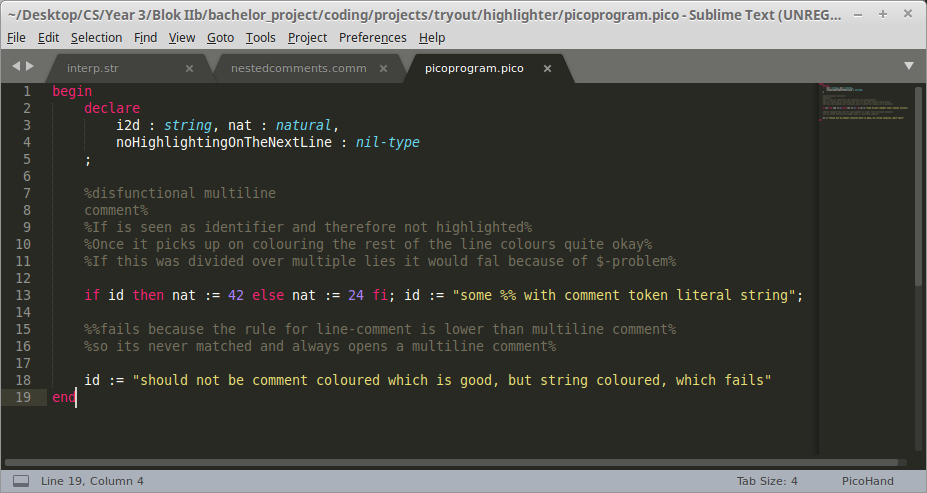
\includegraphics[width=\textwidth, keepaspectratio]{Figures/highlightShots/pico_handwritten.png}
	\decoRule
 	\caption[Hand-written highlighter results for Pico grammar]{Results of the highlighter hand-written for the pico grammar}
\end{figure}

\subsection{Pico breakdown}
In this section I will discuss the results as seen above and point out some of the strong parts and flawed parts of the generated highlighter.\\\\
\textbf{The good:}
\begin{itemize}
\item The parser-like behaviour this highlighter shows ensures that accidents like highlighting "else" in a word like "elsewhere" are practically impossible. When writing the hand-written version the 2 in i2d of that output got coloured as a constant, even though the generated version always gets this right.
\end{itemize}
\textbf{The bad:}
\begin{itemize}
\item The "declaration"-section defines 3 variables. These are \data{id}, \data{nat} and\\ \data{noHighlightingOnTheNextLine}. In this section the highlighter expects rules of the type: \gram{Id ":" Type}, where the type should get the scope \data{storage.type}. This works for the first line, however then it encounters an end-of-line, makes the wrong decision to pop because nothing matches. The next line still contains declarations, but receive no highlighting. This is also true for line 13 and 18, because all of 13 is on one line the highlighting is okay, but it fails at 18 again because of new-lines.\pagebreak
\item "if" is not highlighted because it is seen as an identifier by the highlighter. This is because the match for an Id (any combination of letters, so also "if") is tried earlier than the specific match for if.\\
\begin{lstlisting}[language=SublimeSyntax]
  Statement__DQUOTESEMIDQUOTE__STARSEPS_0:
    - meta_scope: Statement__DQUOTESEMIDQUOTE__STARSEPS_0
      # match for id
    - match: '(?=(([\x{61}-\x{7A}])(([\x{30}-\x{39}\x{61}-\x{7A}])*)(?!([\x{30}-\x{39}\x{61}-\x{7A}]))))'
      set: [Statement__DQUOTESEMIDQUOTE__STARSEPS_1, Id_0]
    - match: '(fi)'
      scope: keyword.control.flow
      set: [Statement__DQUOTESEMIDQUOTE__STARSEPS_2]
    - match: '(while)'
      scope: keyword.control.flow
      set: [Statement__DQUOTESEMIDQUOTE__STARSEPS_6]
    - match: '(else)'
      scope: keyword.control.flow
      set: [Statement__DQUOTESEMIDQUOTE__STARSEPS_4]
    - match: '(od)'
      scope: keyword.control.flow
      set: [Statement__DQUOTESEMIDQUOTE__STARSEPS_5]
      # match for not any of the cases (I.E. non-sink state)
    - match: '(?!((while)|(if)|(else)|(od)|(?=(([\x{61}-\x{7A}])(([\x{30}-\x{39}\x{61}-\x{7A}])*)(?!([\x{30}-\x{39}\x{61}-\x{7A}]))))|(fi)))'
      pop: true
    - match: '(if)'
      scope: keyword.control.flow
      set: [Statement__DQUOTESEMIDQUOTE__STARSEPS_3]
\end{lstlisting}
\item The second "\%" on line 15 is not highlighted because the block-comment match is tried before the line comment match. The block-comment expects a \% then anything that is not \% and then a closing \%. It does not highlight the second \% because it is seen as not part of the comment and the line-comment is too far down the context to be tried.
\begin{lstlisting}[language=SublimeSyntax]
  WhitespaceAndComment_0:
    - meta_scope: WhitespaceAndComment_0
    - match: '(%)'
      scope: comment.block
      set: [WhitespaceAndComment_1]
    - match: '([\x{9}-\x{A}\x{D}\x{20}])'
      pop: true
    - match: '(%%)'
      scope: comment.line
      set: [WhitespaceAndComment_2]
\end{lstlisting}
\end{itemize}


\pagebreak
\subsubsection{Statistics on the final results}
Below are a few tables that show and discuss the performance of the highlighters included in the appendices. They are compared with highlighters that were written by hand. In the appendices there are also examples included of the actual highlights the different versions produce.

\begin{table}[h!]
\caption{Statistics on generated highlighters vs hand-written ones}
\label{tab:highlighters}
\begin{center}
\begin{tabular}{|c|c|c|c|c|}
\hline
\tabhead{Name} & \tabhead{Generated} & \tabhead{SLOC} & \tabhead{NumContexts} & \tabhead{Performance (++/+/-/--)} \\
\hline
Nested comments & true & 100 & 11 & --\\
				& false & 27 & 3 & ++\\
\hline
String Interpolation & true & 77 & 11 & ++\\
					 & false & 33 & 4 & ++\\
\hline
Pico & true & 566 & 57 & -\\
	 & false & 61 & 8 & ++\\
\hline
\end{tabular}
\end{center}
\end{table}
\noindent In here it is clear to see that the parser-like behaviour breaks the highlighter. It introduces many lines and contexts that do not contribute to the performance of the highlighters, only in a negative way.


\section{Overall results}
As can be seen in especially the final results, the highlighters do not do a particularly good job. This is mainly due to the following things:
\begin{enumerate}
\item First of all, looking at the nested comment grammar. In converting the strongly regular grammar into machines all elements of a component are put in one machine. In order to properly highlight nested comments a structure like this is needed: On start of new comment $\rightarrow$ push new machine that highlights a comment. On ending of a comment $\rightarrow$ pop the current machine. This is what the stack is useful for, to keep track of how many times the highlighter is nested. However because of the merging of all comments into one machine and the way the $ToContexts$ part is constructed a new machine is only pushed if the highlighter moves from one machine to one that is outside of its current component (I.E. a non-terminal arc). This never occurs for the nested comment case and this is why it accepts endless amounts of opening and closing comments without ever pushing nor popping machines. (\ref{sec:results:strReg2machines})
\pagebreak\item There is also the issue discussed in \ref{sec:SublimeSyntax:LineEndings} that brings problems in the final algorithm. Since the pushing of new machines is triggered on lookahead of one of the starting tokens of that machine, problems arise when end of lines (\$) are the next token to be consumed. The Sublime highlighter matches per-line, so never past an end of line. Let us assume a highlighter has the following context:
\begin{lstlisting}[language=SublimeSyntax]
context1_A:
  - match: '?=(a)'
    set: [context1_B, context2_A]
  - match: '?!(a)'
    pop: true
\end{lstlisting}
If we have input of the type \data{bla bla\|\$a b c} and the highlighter is at |. The highlighter will now check and try the matches of the context in order. The first one fails, because it can't look past a new-line, since it matches one line at a time. Therefore it will arrive at the final match and pop the context off, even though the real next token is $a$ and therefore the highlighter "should" push the next machine on top. This can be seen in the $Pico$ example program as well.
\item A general problem with the approach as a whole is that the algorithm tries to retain as much of the original structure of the grammar as possible. However when looking at hand-written highlighters, those programs do not really care about the grammar, it just searches for words to match and colour them. In other words, the generated highlighters act as parsers. This is bad for a multitude of reasons:
\subitem \textbf{a}. Highlighting will not continue properly once past a syntax error.\\
		(E.G. keyword in a "wrong" place will get no highlighting)
\subitem \textbf{b}. Normal highlighters just skip tokens that do not need highlighting. It simply continues past them. On matching something it colours correspondingly. The parser-like behaviour wants to match every token it encounters otherwise it does not continue to the next context. This is bad for a simple reason: more meaningless matching and trying leads to a larger chance of errors.
\subitem \textbf{c}. It introduces the shift-reduce and reduce-reduce like conflicts found when the highlighter is in the final state of a machine. Even though highlighters should easily be able to highlight grammars outside $LR(1)$. It ensures the need for something like $solveConflicts$, which as been shown to be the reason the algorithm does not perform on large grammars.
\item The last problem is more of a beauty remark. The created highlighters are huge and get out of hand fairly soon. A highlighter that was generated for an 80-line grammar describing JSON objects, generated a highlighter of over 750 lines of code. One can only imagine if this were run on for example the C-language.
\end{enumerate}


